\subsection{Ist-Analyse}
\label{sec:IstAnalyse}

Momentan lassen sich Informationen über die angebotenen Studiengänge am
Stu\-di\-en\-stand\-ort Lingen über die Hochschulseite
\url{www.hs-osnabrueck.de} abrufen. Diese Internetseite bietet dabei
weiterführende Links mit Informationen für Studierende und Unternehmen. Hier
werden unter anderem Labore, Projekte und Dozenten der Hochschule vorgestellt.
Darüber hinaus werden in einer Bildergalerie einzelne Impressionen des neuen
Campus präsentiert. Ein Bildschirmfoto dieser Internetseite ist in
\abbildung{Bildergalerie} abgebildet.

\begin{figure}[htb]
\centering
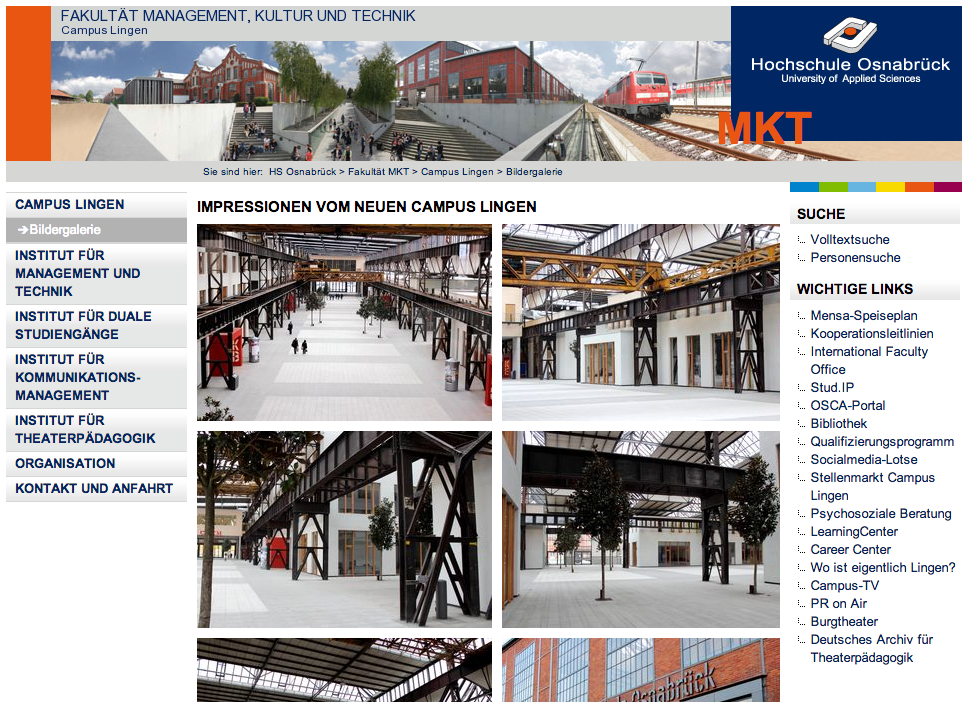
\includegraphics[width=1.0\textwidth]{Bildergalerie.png}
\caption[Bildergalerie des Campus Lingen]{Bildergaliere des Campus Lingen\protect\footnotemark}
\label{fig:Bildergalerie}
\end{figure}
\footnotetext{Darstellung entnommen von
\url{http://www.campus-lingen.hs-osnabrueck.de}}

Ähnlich wie die Informationsvermittlung auf der Internetseite der Hochschule
Osnabrück gestaltet sich auch die Informationsvermittlung auf Messen. Diese
Messen bieten Studieninteressierten die Möglichkeit, sich über die einzelnen
Studienangebote zu erkundigen. Auf den Messen werden ebenfalls einzelne
Impressionen des neuen Campus in Lingen gezeigt und Informationsmaterial hierzu
verteilt.

Im Zuge dieser Analyse wurden zwei Elemente heraugestellt, welche eventuell vor
dem Hintergrund der Projektidee wiederverwendet werden können.

\begin{enumerate}
  \item Bereits aufgenommene Fotos vom Campus Lingen, welche auf der
  Internetseite präsentiert werden.
  \item Das Informationsmaterial das über Projekte, Studiengänge, Dozenten und
  weiteres zusammengetragen wurde.
\end{enumerate}

Die bereits angefertigen Fotos können dabei nicht für das vorliegende Projekt
verwendet werden, da es sich bei den Fotos nicht um 360-Grad-Fotos handelt.
Darüber hinaus sind auf diesen Fotos nur einzelne Impressionen des Campus
dargestellt und keine umfassenden Einblicke. Die bestehenden Impressionen
zeigen jedoch interessante Blickwickel des Campus. Diese Blickwinkel können bei
der Erstellung der neuen 360-Grad-Fotos aufgegriffen werden.

Das auf der Internetseite der Hochschule zusammengetragene Informationsmaterial
kann hingegen in dem Projekt wiederverwendet werden. Die Informationen können
360-Grad-Fotos im Projekt zugeordnet und zusammen mit diesen angezeigt werden.
Weiterhin kann auf die bereits bestehenden Informationen auf der Internetseite
der Hochschule verlinkt werden. Für die Rechereche nach Informationsmaterial im
Projekt kann auf diese Weise Aufwand eingespart werden.